\section{Marco teórico}

\subsection{El problema del plegamiento de proteínas}
\label{sec:plegamiento}

Una proteína se sintetiza como una cadena lineal de aminoácidos unidos por enlaces peptídicos. Cada aminoácido tiene una cadena lateral distinta, y algunas de estas cadenas laterales interactúan bien con el agua (son polares o tienen carga) mientras que otras la evitan (son hidrofóbicas). Al quedar en solución, la cadena se dobla sobre sí misma hasta alcanzar una forma tridimensional estable, llamada estado nativo, y es esa forma la que le permite cumplir su función biológica.

Los experimentos de Anfinsen con la ribonucleasa mostraron que una proteína desnaturalizada recupera por sí sola su forma activa cuando se regresan las condiciones normales. De ahí surgió la llamada hipótesis termodinámica: la información necesaria para plegarse está contenida en la secuencia, y el estado nativo corresponde a la conformación de mínima energía libre~\cite{anfinsen1973principles}. Esta hipótesis convierte el plegamiento en un problema de optimización: dada una secuencia, encontrar la conformación que minimiza una función de energía.

Entre las fuerzas que intervienen, la más importante para el plegamiento global es el efecto hidrofóbico~\cite{kauzmann1959some, dill1990dominant}. Los aminoácidos hidrofóbicos tienden a agruparse en el interior de la proteína, lejos del agua, y los polares quedan en la superficie. En muchas proteínas globulares este núcleo hidrofóbico es la característica estructural más clara.

El problema es difícil incluso para la propia proteína si se piensa en términos de búsqueda. Levinthal hizo notar que si una cadena de unos cien aminoácidos probara sus conformaciones una por una, aun a gran velocidad, tardaría más que la edad del universo en encontrar la correcta, y sin embargo las proteínas reales se pliegan en milisegundos o segundos~\cite{levinthal1969fold}. Esto se conoce como la paradoja de Levinthal, y muestra que la cadena sigue un paisaje de energía que la guía hacia el estado nativo sin probar todas las conformaciones. Para un algoritmo, que no tiene esa guía física, el tamaño del espacio de conformaciones sí es el obstáculo principal.

Hoy existen métodos de aprendizaje profundo, como AlphaFold, que predicen la estructura de muchas proteínas con una precisión cercana a la experimental~\cite{jumper2021alphafold}. Estos métodos aprenden de miles de estructuras conocidas y no resuelven el problema de optimización de forma explícita. Los modelos simplificados como el HP siguen siendo útiles para estudiar el problema de búsqueda en sí mismo y para comparar algoritmos de optimización en condiciones controladas.

%%%%%%%%%%%%%%%%%%%%%%%%%%%%%%%%%%%%%%%%%%%%%%%%%%%%%
\subsection{El modelo HP}
\label{sec:modelo_hp}

El modelo hidrofóbico-polar fue propuesto por Dill~\cite{dill1985theory} y estudiado en detalle por Lau y Dill~\cite{lau1989lattice}. Conserva solo el efecto hidrofóbico y hace tres simplificaciones:

\begin{enumerate}
    \item Los 20 aminoácidos se reducen a dos clases: hidrofóbicos (H) y polares (P). Una proteína se describe entonces con una cadena $s = s_1 s_2 \cdots s_n$, con $s_i \in \{H, P\}$.
    \item La cadena se coloca sobre una red regular. En esta práctica usamos la red cuadrada en dos dimensiones, así que cada aminoácido ocupa un punto de coordenadas enteras.
    \item La energía solo cuenta los contactos entre aminoácidos H.
\end{enumerate}

Una conformación es una asignación de posiciones $\mathbf{p}_1, \dots, \mathbf{p}_n \in \mathbb{Z}^2$ que cumple dos condiciones. La primera es que aminoácidos consecutivos ocupen puntos vecinos de la red, $\lVert \mathbf{p}_{i+1} - \mathbf{p}_i \rVert = 1$. La segunda es que dos aminoácidos no ocupen el mismo punto, $\mathbf{p}_i \neq \mathbf{p}_j$ si $i \neq j$. A un recorrido con estas propiedades se le llama \textit{caminata autoevitante}.

Dos aminoácidos $i$ y $j$ forman un \textit{contacto topológico} si están en puntos vecinos de la red pero no son consecutivos en la cadena ($|i - j| > 1$). La energía de una conformación $C$ es
\begin{equation}
E(C) = \sum_{i < j - 1} \varepsilon(s_i, s_j)\, \Delta(i, j),
\qquad
\varepsilon(s_i, s_j) =
\begin{cases}
-1 & \text{si } s_i = s_j = H,\\
\phantom{-}0 & \text{en otro caso,}
\end{cases}
\label{eq:energia_hp}
\end{equation}
donde $\Delta(i,j) = 1$ si $\mathbf{p}_i$ y $\mathbf{p}_j$ son vecinos en la red y 0 si no lo son. En otras palabras, la energía es menos el número de contactos H-H. El problema consiste en encontrar la conformación $C^*$ que minimiza $E$, que en este modelo se toma como el estado nativo.

Los pares consecutivos no se cuentan porque siempre están juntos, sin importar cómo se doble la cadena, y por lo tanto no distinguen una conformación de otra. Los contactos con aminoácidos P tampoco aportan energía. La Figura~\ref{fig:modelo_hp} muestra la misma cadena de ocho aminoácidos estirada y plegada: la cadena estirada no tiene contactos H-H, mientras que al doblarla la primera H queda junto a la última y la tercera junto a la sexta, con lo que la energía baja a $-2$.

\begin{figure}[H]
\centering
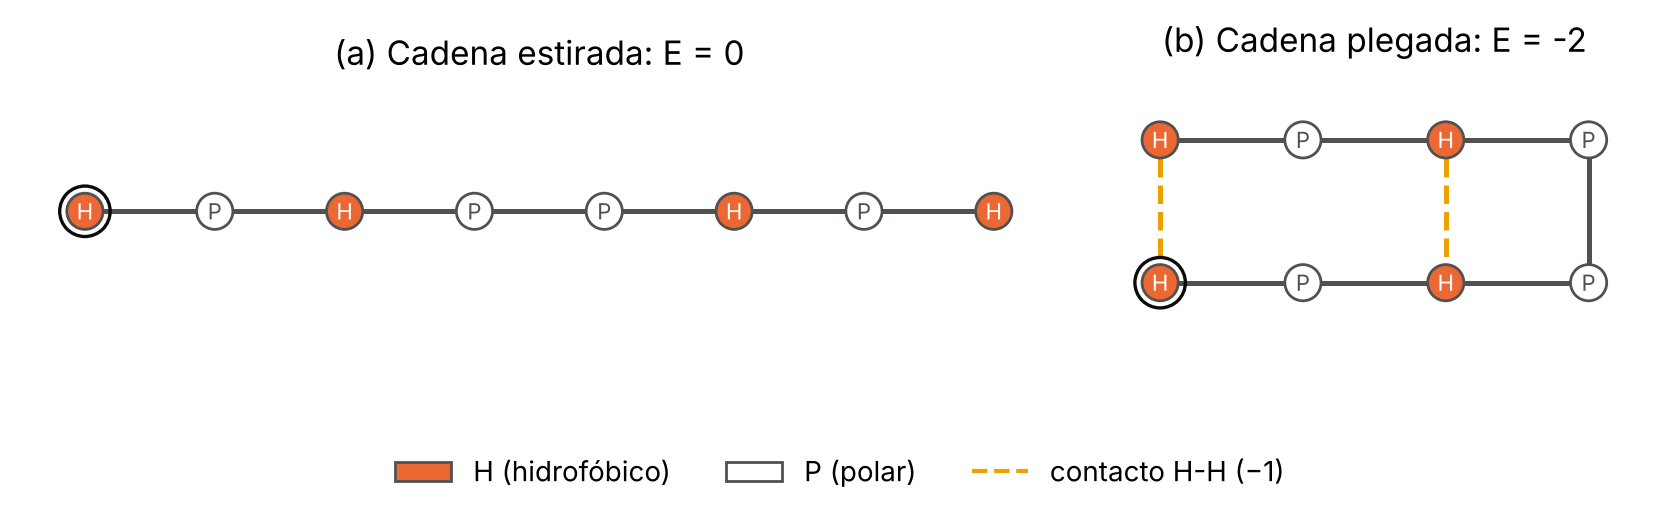
\includegraphics[width=0.95\textwidth]{figuras/hp_modelo_ejemplo.png}
\caption{La secuencia HPHPPHPH en dos conformaciones. El círculo negro marca el primer aminoácido. (a) Estirada, sin contactos H-H. (b) Plegada en un rectángulo de $2 \times 4$, con dos contactos H-H (líneas punteadas).}
\label{fig:modelo_hp}
\end{figure}

En una red cuadrada, cada aminoácido interior de la cadena tiene cuatro vecinos en la red, y dos de ellos ya están ocupados por sus vecinos en la cadena. Por eso un aminoácido interior puede formar a lo más dos contactos, y uno de los extremos a lo más tres. Además, la red cuadrada es bipartita (se puede colorear como un tablero de ajedrez), y dos puntos vecinos siempre tienen colores distintos. Como los aminoácidos de posición par e impar alternan colores a lo largo de la cadena, solo pueden formar contacto un aminoácido en posición par con uno en posición impar. Estas restricciones limitan cuántos contactos puede tener una cadena, pero no dicen cómo conseguirlos.

%%%%%%%%%%%%%%%%%%%%%%%%%%%%%%%%%%%%%%%%%%%%%%%%%%%%%
\subsection{Por qué el problema es tan difícil}
\label{sec:dificultad}

\subsubsection{Tamaño del espacio de búsqueda}

El número de conformaciones posibles de una cadena es el número de caminatas autoevitantes de $n-1$ pasos. Para la red cuadrada no se conoce una fórmula cerrada, pero se sabe que crece de forma exponencial,
\begin{equation}
c_m \sim A\, \mu^{m}\, m^{\gamma - 1},
\label{eq:saw}
\end{equation}
donde $c_m$ es el número de caminatas de $m$ pasos, $\mu \approx 2.638$ es la constante de conectividad de la red cuadrada y $\gamma = 43/32$~\cite{jensen2004enumeration}. La constante $\mu$ es un poco menor que 3 porque, después del primer paso, cada nuevo paso tiene a lo más tres opciones (no puede regresar sobre el anterior), y algunas de ellas chocan con la propia cadena. Para una cadena de 100 aminoácidos, $\mu^{99} \approx 5 \times 10^{41}$, así que la búsqueda exhaustiva es imposible incluso para cadenas de tamaño moderado.

\subsubsection{Complejidad computacional}

El tamaño del espacio no basta para decir que un problema es difícil: hay problemas con espacios enormes que se resuelven de forma eficiente. En el caso del modelo HP, Crescenzi et al.~\cite{crescenzi1998complexity} demostraron que encontrar la conformación de mínima energía en la red cuadrada bidimensional es NP-completo, y Berger y Leighton~\cite{berger1998protein} demostraron lo mismo para la red cúbica en tres dimensiones. Esto significa que no se conoce un algoritmo que garantice encontrar el óptimo en tiempo polinomial, y que encontrarlo para cualquier cadena sería tan difícil como resolver cualquier otro problema de la clase NP. En la práctica se usan métodos exactos para cadenas cortas y metaheurísticas para las largas.

\subsubsection{Forma del paisaje de energía}

Además del tamaño, la forma de la función objetivo dificulta la búsqueda:

\begin{itemize}
    \item La energía solo toma valores enteros entre 0 y un mínimo pequeño (por ejemplo, $-9$ para una cadena de 20 aminoácidos). Millones de conformaciones distintas comparten la misma energía, así que el paisaje está formado por grandes mesetas. Dentro de una meseta, la energía no da ninguna pista sobre hacia dónde moverse.
    \item Un cambio pequeño en la conformación, como cambiar la dirección de un solo paso, puede mover toda la parte final de la cadena y destruir muchos contactos a la vez. Dos conformaciones parecidas en su descripción pueden tener energías muy distintas.
    \item Una fracción grande de las descripciones posibles produce cadenas que se cruzan consigo mismas y no son conformaciones válidas. Esta fracción aumenta con la longitud de la cadena (lo medimos en la Sección~\ref{sec:representacion}).
    \item La conformación óptima casi nunca es única. Además de las rotaciones y reflexiones, que siempre dan ocho copias equivalentes de cada conformación en la red cuadrada, puede haber conformaciones realmente distintas con la misma energía mínima.
\end{itemize}

\subsubsection{Cadenas de referencia}

Para comparar algoritmos se usa un conjunto de secuencias de prueba en dos dimensiones, de 20 a 100 aminoácidos, introducido por Unger y Moult~\cite{unger1993genetic} y usado después en muchos trabajos, entre ellos el algoritmo de colonia de hormigas de Shmygelska y Hoos~\cite{shmygelska2005ant}. Para cada secuencia se reporta la mejor energía conocida $E^*$. En las cadenas cortas esa energía se ha demostrado óptima; en las largas es el mejor valor encontrado hasta ahora por algún método. Los métodos que alcanzan esos valores en cadenas largas suelen combinar una búsqueda global con movimientos locales especializados, como los \textit{pull moves} de Lesh et al.~\cite{lesh2003complete}, que jalan un segmento de la cadena a una nueva posición sin romperla.

%%%%%%%%%%%%%%%%%%%%%%%%%%%%%%%%%%%%%%%%%%%%%%%%%%%%%
\subsection{Representación de conformaciones}
\label{sec:codificaciones}

Para usar un algoritmo de búsqueda hay que describir cada conformación con una lista de símbolos o números. Como el primer aminoácido puede fijarse en el origen, basta con dar la dirección de cada paso. Krasnogor et al.~\cite{krasnogor1999protein} compararon las dos formas habituales de hacerlo:

\begin{itemize}
    \item \textit{Codificación absoluta}: cada paso es una dirección fija de la red (arriba, abajo, izquierda o derecha). Hay cuatro opciones por paso, y una de ellas siempre es inválida porque regresa sobre el aminoácido anterior.
    \item \textit{Codificación relativa}: cada paso se describe respecto a la dirección del paso anterior (girar a la izquierda, seguir de frente o girar a la derecha). Hay tres opciones por paso y ninguna regresa sobre el paso anterior.
\end{itemize}

Con la codificación relativa el espacio de búsqueda pasa de $4^{n-1}$ a $3^{n-2}$ descripciones (el segundo aminoácido se fija también, porque rotar toda la cadena no cambia su energía). Las dos codificaciones también difieren en el efecto de un cambio: con la relativa, cambiar un paso gira todo el resto de la cadena alrededor de ese punto, mientras que con la absoluta lo traslada, y eso cambia qué conformaciones quedan ``cerca'' unas de otras para el algoritmo~\cite{krasnogor1999protein}. Ninguna de las dos codificaciones impide que la cadena choque consigo misma a más de un paso de distancia, así que cada algoritmo debe decidir qué hacer con esas descripciones inválidas: descartarlas, penalizarlas o repararlas.

%%%%%%%%%%%%%%%%%%%%%%%%%%%%%%%%%%%%%%%%%%%%%%%%%%%%%
\subsection{Optimización por enjambre de partículas}
\label{sec:pso}

PSO fue propuesto por Kennedy y Eberhart en 1995, inspirado en el movimiento coordinado de bandadas de aves~\cite{kennedy1995pso}. Cada partícula $i$ tiene una posición $X_i$, que representa una solución, y una velocidad $V_i$. Guarda además la mejor posición que ha visitado, $P_i$ (\textit{pbest}), y conoce la mejor posición encontrada por todo el enjambre, $G$ (\textit{gbest}). En cada iteración se actualizan con~\cite{shi1998modified}:
\begin{align}
V_{id}(t+1) &= w\,V_{id}(t) + c_1 r_1 \left(P_{id} - X_{id}(t)\right) + c_2 r_2 \left(G_d - X_{id}(t)\right), \label{eq:velocidad}\\
X_{id}(t+1) &= X_{id}(t) + V_{id}(t+1), \label{eq:posicion}
\end{align}
donde $d$ es la dimensión y $r_1$, $r_2$ son números aleatorios uniformes en $[0,1]$. El peso de inercia $w$ controla cuánto conserva la partícula su movimiento anterior; un valor alto favorece la exploración de regiones nuevas y uno bajo la concentra cerca de las soluciones conocidas~\cite{shi1998parameter}. El coeficiente cognitivo $c_1$ atrae a cada partícula hacia su propio \textit{pbest}, y como cada partícula tiene uno distinto, mantiene la variedad del enjambre. El coeficiente social $c_2$ atrae a todas hacia el mismo \textit{gbest}, lo que acelera la convergencia y reduce la variedad~\cite{ratnaweera2004self}.

\subsubsection{Coeficientes variables}

Al inicio de la búsqueda conviene explorar y al final conviene refinar~\cite{crepinsek2013exploration}. Shi y Eberhart propusieron reducir $w$ de forma lineal de 0.9 a 0.4~\cite{shi1999empirical}, y Ratnaweera et al. aplicaron la misma idea a los coeficientes de aceleración, disminuyendo $c_1$ de 2.5 a 0.5 y aumentando $c_2$ de 0.5 a 2.5 (esquema TVAC)~\cite{ratnaweera2004self}. La variación no tiene que ser lineal: Chatterjee y Siarry~\cite{chatterjee2006nonlinear} propusieron una inercia que decrece de forma no lineal, y otros trabajos ajustan los coeficientes según el estado de la búsqueda~\cite{zhan2009adaptive, nickabadi2011novel}.

Una curva que se usa mucho para variar un parámetro de forma no lineal es el decaimiento coseno, popularizado en el entrenamiento de redes neuronales por Loshchilov y Hutter, quienes además lo combinan con reinicios periódicos~\cite{loshchilov2017sgdr}. Para un avance normalizado $s \in [0,1]$,
\begin{equation}
g(s) = \tfrac{1}{2}\left(1 + \cos(\pi s)\right)
\label{eq:coseno}
\end{equation}
va de 1 a 0, cambiando despacio al principio y al final y rápido a la mitad.

\subsubsection{Estabilidad}

No cualquier combinación de coeficientes produce un enjambre que converge. Poli~\cite{poli2009mean} analizó la media y la varianza de la posición de una partícula y obtuvo que su distribución se estabiliza si
\begin{equation}
c_1 + c_2 < \frac{24\,(1 - w^2)}{7 - 5w}.
\label{eq:poli}
\end{equation}
Si la condición no se cumple, las partículas siguen oscilando con amplitud creciente (limitada en la práctica por la velocidad máxima), lo que equivale a una exploración amplia.

%%%%%%%%%%%%%%%%%%%%%%%%%%%%%%%%%%%%%%%%%%%%%%%%%%%%%
\subsection{Diversidad del enjambre}
\label{sec:diversidad}

La diversidad mide qué tan dispersas están las partículas y permite observar el paso de la exploración a la explotación~\cite{olorunda2008measuring}. Usamos la distancia promedio de cada vector al centroide:
\begin{equation}
D(\mathbf{v}_1, \dots, \mathbf{v}_N) = \frac{1}{N} \sum_{i=1}^{N} \left\lVert \mathbf{v}_i - \bar{\mathbf{v}} \right\rVert, \qquad \bar{\mathbf{v}} = \frac{1}{N}\sum_{i=1}^{N} \mathbf{v}_i,
\label{eq:diversidad}
\end{equation}
aplicada a tres conjuntos de vectores. La \textit{diversidad de posición} usa las posiciones actuales $X_i$ e indica qué tan repartido está el enjambre. La \textit{diversidad de velocidad} usa las velocidades $V_i$; cuando tiende a cero, las partículas se mueven igual o ya no se mueven. La \textit{diversidad cognitiva} usa las mejores posiciones personales $P_i$ e indica qué tan distintos son los ``recuerdos'' de las partículas; como $P_i$ solo cambia cuando la partícula mejora, esta medida cambia más despacio que las otras dos.

%%%%%%%%%%%%%%%%%%%%%%%%%%%%%%%%%%%%%%%%%%%%%%%%%%%%%
\subsection{Prueba de Mann-Whitney}
\label{sec:mannwhitney}

Para decidir si un algoritmo es mejor que otro no basta una ejecución, porque PSO es estocástico. Se ejecuta cada versión varias veces y se comparan las muestras con una prueba no paramétrica, ya que los resultados de las metaheurísticas rara vez siguen una distribución normal~\cite{derrac2011practical}. La prueba de Mann-Whitney~\cite{mann1947test} compara dos muestras independientes: junta los valores de ambas, los ordena, les asigna rangos y calcula el estadístico
\begin{equation}
U = R_1 - \frac{n_1 (n_1 + 1)}{2},
\end{equation}
donde $R_1$ es la suma de los rangos de la primera muestra y $n_1$ su tamaño. Si las dos muestras vienen de la misma distribución, $U$ debe quedar cerca de $n_1 n_2 / 2$. En la versión unilateral que usamos, la hipótesis alternativa es que los valores de la primera muestra tienden a ser menores que los de la segunda, y la hipótesis nula se rechaza si el valor $p$ es menor que $\alpha = 0.05$. Como la energía del modelo HP solo toma valores enteros, hay muchos empates; la prueba los maneja asignando a los valores empatados el promedio de sus rangos.
